% ----------------------------------------------------------------------------
% thesis.tex:	Template for Master Thesis and PhD Dissertation
%             Northeastern University, Electrical and Computer Engineering
%
% This document contains embedded instructions. Each instruction line starts
% with "%%", conversely code options to enable, only start with a single "%"
% ----------------------------------------------------------------------------
% edited by:	Gunar Schirner
% last update:	see SVN
% ----------------------------------------------------------------------------

%% Options
%% PHD    -- PhD Dissertation (default: MS Thesis)
%% draft  -- label as draft version (default: final)
%% Remove [PHD] if MS Thesis
\documentclass[]{macro/neu_msthesis}

% --- Global Definitions for title and others ---

%% define thesis title
\title{Super-Convincing Thesis Title}

%% define thesis author
\author{Hubert Husky}
\nuid{123456789}

%% department name
\dept{Electrical and Computer Engineering}

%% degree name if not "Master of Science" or "Doctor of Philosophy"
%% should not be needed
%\degree{My Custom Degree Name}

%% area of degree
%% will be used on degree page:
%% For MS students "Electrical and Computer Engineering"
%% For PhDEE students "Electrical Engineering"	
%% For PhDCE students "Computer Engineering"
\degreename{Electrical and Computer Engineering}

%% General field in which degree is obtainded (usually same as \degreename{})
\field{Electrical and Computer Engineering}

%% Define month when submitted (START writing early or it will be very soon too late :-) )
%% Use full name for months
\submitdate{December 2014}

%% how many committee members (including adviser, put a number between 3 and 6)
\numberofmembers{3}

%% Define committee member names, except for the advisor, all other names come in alphabetical order (last name)
\principaladviser{Dr. Advisor}
\firstreader{Dr. First Member}
\secondreader{Dr. Second Member}

\thirdreader{Dr. Third Member}
\fourthreader{Dr. Fourth Member}
\fifthreader{Dr. Fifth Member}

%% name chair of department
\chairman{Dr. Sheila Hemami}

%% name of director graduate school
\dean{Dr. Sara Wadia-Fascetti}

%% all user defined macros
%% outsourced conveniently to keep this file clean
% a set of default macros (outsourced of main document for cleanliness


\usepackage{amsfonts,amssymb,amsmath}			% special math characters
\usepackage{times}		% use Postscript fonts
\usepackage{bm}


% reference macros (capitals!)
\newcommand{\figref}[1]{Figure~\ref{#1}}
\newcommand{\tabref}[1]{Table~\ref{#1}}
\newcommand{\chapref}[1]{Chapter~\ref{#1}}
\newcommand{\secref}[1]{Section~\ref{#1}}
\newcommand{\appref}[1]{Appendix~\ref{#1}}
\newcommand{\lineref}[1]{line~\ref{#1}}
\newcommand{\Lineref}[1]{Line~\ref{#1}}

\newcommand{\ifyes}[1]{#1}
\newcommand{\ifno}[1]{}


% local macro
\usepackage{multirow}
\clubpenalty=1000
\widowpenalty=1000

% misc. settings
\setcounter{secnumdepth}{3}

% enable index generation
\makeindex
\usepackage{makeidx}
\usepackage{acronym}

% format URLs
\usepackage{url}
% default style was sf but it produced a too big font in the reference section
\urlstyle{tt}

% graphics package depending on backend driver
% are we directly producing pdf? ie. running pdflatex ?
\ifnum\pdfoutput>0
\usepackage[pdftex]{graphicx}
% enable on the fly conversion of eps figures when using pdfLatex
\usepackage{epstopdf}
\else
\usepackage{graphicx}
\fi


% ----------------------------------------------------------------- %
% hyperref to create bookmarks in the PDF for easier navigation


% either for pdflatex
\ifnum\pdfoutput>0
\usepackage[pdftex,%                    % hyper-references for ps2pdf
bookmarks=true,%                        % generate bookmarks ...
bookmarksnumbered=true,%                % ... with numbers
hypertexnames=false,%                   % needed for correct links to figures
breaklinks=true           %Allows link text to break across lines;
]{hyperref}
% or for dvips ..
\else
\usepackage[hypertex,%                  % hyper-references for ps2pdf
bookmarks=true,%                        % generate bookmarks ...
bookmarksnumbered=true,%                % ... with numbers
hypertexnames=false,%                   % needed for correct links to figures
breaklinks=true           %Allows link text to break across lines;
]{hyperref}
\fi


\hypersetup{				% setup PDF information fields
pdfauthor = {\authorRef},
pdftitle = {\titleRef},
pdfsubject = {\expandafter{\degreeRef} thesis submitted to Northeastern University},
pdfkeywords = {add keywords here}
pdfcreator = {LaTeX with hyperref package},
pdfproducer = {dvips + ps2pdf}}

\usepackage{microtype}



% --- begin of document ---
\begin{document}

% add a pdf bookmark to the cover page
\pdfbookmark[1]{Cover}{cover}

% --- title page ---
\titlepage

% --- front matter ---
\begin{frontmatter}
% print signature page
\signaturepage
% dedication
% dedication.tex:

\begin{dedication}
To my family.
\end{dedication}


% table of content (add bookmark for convenience)
\pdfbookmark[1]{Table of Contents}{contents}
\tableofcontents
\listoffigures
\newpage\ssp
\listoftables

% include a list of Acronyms (comment out if no acronyms are specified)
% acronyms.tex

\chapter*{List of Acronyms}
\addcontentsline{toc}{chapter}{List of Acronyms}

% below is the list of acronym definitions, place them in alphabetical order
% since they will not be sorted again. 
\begin{acronym}
\acro{AHB}{Advanced High-performance Bus}.
	System bus definition within the AMBA 2.0 specification. Defines a high-performance bus including pipelined access, bursts, split and retry operations.

\acro{ATLM}{Arbitrated Transaction Level Model}.
  A model of a system in which communication is described as transactions, abstract of pins and wires.
  In addition to what is provided by the \acs{TLM}, it models arbitration on a bus transaction level.
\acro{TLM}{Transaction Level Model}.
  A model of a system in which communication is described as transactions, abstract of pins and wires.


\end{acronym}


%% include any of the front matter files that contain text
%% attention the input does cause a page break, the include on
%% the other hand does not
% acknowledgements.tex:

\begin{acknowledgements}

Here I wish to thank those who have supported me during the process of the thesis work.... 
\end{acknowledgements}


% abstract.tex:

\begin{abstract}

This is a very abstract abstract.

\end{abstract}



\end{frontmatter}


% --- body of the document ---
\pagestyle{headings}

%% include each chapter like below
% intro.tex:

\chapter{Introduction}
\label{chap:intro}
This is where the intro goes.
There is a planet ... where people still believe digital watches are the
greatest invention. It is mostly harmless.

\section{Life, Universe and Everything}
\label{chap:intro:design}

Simple, quantitative answers to the most pondering questions are beautiful. More about question of life, universe and everything can be found in \cite{book:42}.

This is where the text goes. One can refer to a previous chapter like \chapref{chap:intro}. To find all the other reference possibilities search in the MACROS folder for chapref. Also one can include pictures, preferably in the pdf format like shown in \figref{fig:intro:meth}. Graphics can also be included as eps, if graphics is in eps, the epstopdf packages converts it to pdf on the fly. See examples below in \figref{fig:intro:meth2}.

To keep the code clean, call all extra packages that you would like to use from the file macro.tex in the macro folder. Also keep all your graphics in the fig folder and all bibliography related files in the bib folder.

Make sure that you run bibtex and makeindex to geberate bibliography and index.

This demonstrates how to include a term\index{Term} into the index\index{Index}. For details, check out \cite{latex:index}.

\begin{figure}[htbp]
  \centering
    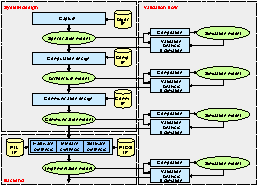
\includegraphics[width=0.5\textwidth]{fig/meth.pdf}
  \caption[Design methodology for SoC design]{\label{fig:intro:meth} Design methodology for SoC design (Source \cite{book:SpecC:yellow})}
\end{figure}

\begin{figure}[htbp]
  \centering
    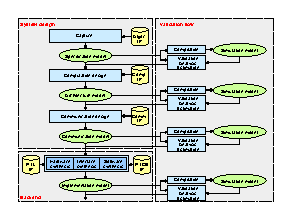
\includegraphics[width=0.5\textwidth]{fig/meth.eps}
  \caption{\label{fig:intro:meth2} Design methodology but included as EPS figure}
\end{figure}

Also tables are possible as shown in \tabref{tab:ConclusionSummary}. What is really cool are the acronyms. The first time you use one, like \ac{TLM} then it appears with full description. Using it the second time makes only the acronym appears \ac{TLM}.

\begin{table}[htbp]
  \centering
     \begin{tabular}{|l|c|}
        \hline
         \textbf{Environment Condition} & \textbf{Applicable Model} \\
			\hline
			 \begin{tabular}{@{}l@{}}
			 $\bullet\,$ single master bus \\
			 $\bullet\,$ no overlap between masters bus access\\
			 \end{tabular}
			&
			 \ac{TLM}
			\\
			\hline
			 \begin{tabular}{@{}l@{}}
			 $\bullet\,$ only locked transfers \\
			 $\bullet\,$ unlocked transfers and low overlap\\
			 \end{tabular}
			&
			 \ac{ATLM}
			\\
			\hline
			 \begin{tabular}{@{}l@{}}
			 $\bullet\,$ unlocked transfers and high overlap\\
			 \end{tabular}
			&
			 bus functional
			\\
			\hline
		\end{tabular}
	\caption{Conclusion summary}
	\label{tab:ConclusionSummary}
\end{table}

Now time for some math\index{Math}:
\begin{align}
F(x)&=\int_{-\infty}^x f(u)\,du\\
\bm{Ax}&=\bm{b}\\
\mathbf{Ax}&=\mathbf{b}\\
\sin^2(\theta)+\cos^2(\theta)&=1\\
x&\in\mathcal{X}
\end{align}

The difference in using \verb1\bm1  and \verb1\mathbf1  is clear from above.
% --- EOF ---


%% background
%\input{tex/background.tex}

%% conclusion
\chapter{Conclusion}
\label{chap:conclude}

Writing a long manuscript is easy ... only if one starts early enough. 



% --- Bibliography ----
\bibliographystyle{ieeetran}

%% include bibliography definition
\bibliography{bib/thesis}


% --- Appendix ---
\appendix
%%include anything you need in the appendix
%\include{appendix/appendix}


% --- Index ----
\printindex


% --- that's it ---
\end{document}

% --- EOF --------------------------------------------------------------------

